\documentclass[11pt]{article} 

\usepackage{amssymb,amsmath} 
\usepackage{graphicx}
\usepackage[section]{placeins}
\usepackage{perpage}
\MakePerPage{footnote}


\begin{document}
	\title{STA 511 Homework \#6}
	\date{December 8}
	\author{Suruchi Jaikumar Ahuja}
	\maketitle
	\renewcommand{\thefootnote}{\arabic{footnote}}

\begin{enumerate}

\item Question 1
\begin{enumerate}

\item Given g(x) = ${\dfrac{\theta}{2} }e^{-\theta|x|}$ for $\theta > 0$;\\
f(x) is the standard normal pdf and is given by f(x) =$ \dfrac{1}{\sqrt{2\pi}} e^\frac{-x^2}{2}$\\
For optimal $\theta$ refer to Figure 1.\footnotemark 
			\footnotetext{Refer Appendix 1a for the R code for optimal rejection constant.} \\

\begin{figure}[h]
	\caption[Figure1]{Optimal $\theta$ value}
    \centering
     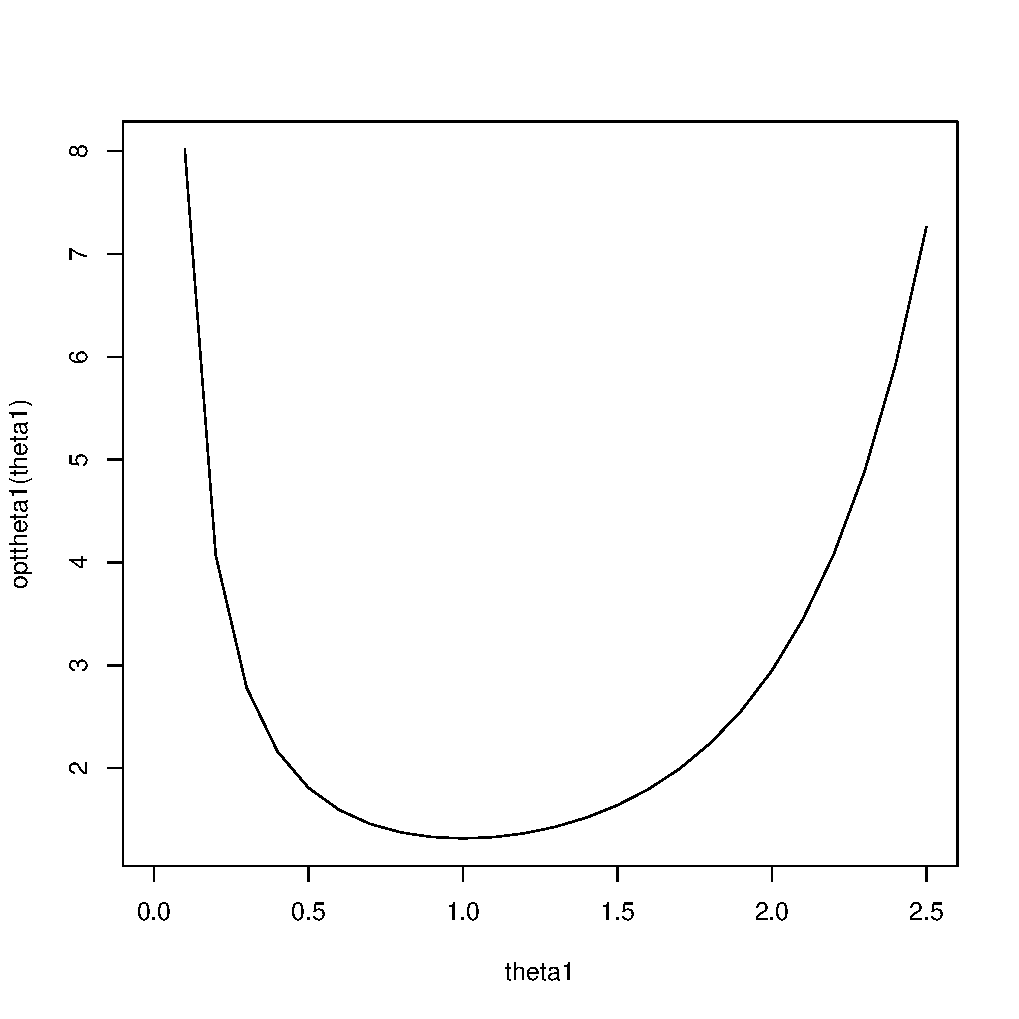
\includegraphics[scale=0.4]{1q.pdf}
      \label{fig1}			
\end{figure}

                                   $$c= sup\dfrac{f(x)}{g(x)}$$\\
                                   $$= sup\dfrac{\dfrac{1}{\sqrt{2\pi}} e^\frac{-x^2}{2}}{{\dfrac{\theta}{2} }e^{-\theta|x|}}$$\\
                                   $$ = \dfrac{1}{\sqrt{2\pi}}\dfrac{2}{\theta} e^{-\frac{x^2}{2}+\theta|x|}$$\\
    So,
\begin{equation*}
c \rightarrow
\begin{cases}
\frac{1}{\sqrt{2\pi}}\frac{2}{\theta} e^{-\frac{x^2}{2}+\theta(x)} if x \geq 0\\
\frac{1}{\sqrt{2\pi}}\frac{2}{\theta} e^{-\frac{x^2}{2}-\theta(x)} if x < 0 \\
\end{cases}
\end{equation*}\\

Now setting the dervatives to zero,

$ \dfrac{d}{dx}  \dfrac{1}{\sqrt{2\pi}}\dfrac{2}{\theta} e^{-\frac{x^2}{2}+\theta(x)} =^{set} 0$  if $x \geq 0\\$\\
$\dfrac{d}{dx}    \dfrac{1}{\sqrt{2\pi}}\dfrac{2}{\theta} e^{-\frac{x^2}{2}-\theta(x)}  = ^{set} 0$ if $x < 0 \\$

$\rightarrow \sqrt{\dfrac{2}{\pi \theta^2}} e^{-\frac{x^2}{2}+\theta x}(-x+\theta) = 0 $ if $x \geq 0$\\
$ \rightarrow \sqrt{\dfrac{2}{\pi \theta^2}} e^{-\frac{x^2}{2}+\theta x}(-x - \theta) = 0 $ if $x < 0 \\$


Now, the critical points are chosen as 
$$ x = \theta for x \geq \theta$$
$$x = - \theta for  x < \theta $$\\

$c_{\theta} = \sqrt{\dfrac{2}{\pi \theta^2}} e ^{-\frac{\theta^2}{2}+\theta^2} \rightarrow \sqrt{\dfrac{2}{\pi \theta^2}}e^{\frac{\theta^2}{2}} $ for $ x \geq 0 $\\
And, \\
$c_{\theta} = \sqrt{\dfrac{2}{\pi \theta^2}} e ^{-\frac{(-\theta^2)}{2}- \theta(-\theta)} \rightarrow \sqrt{\dfrac{2}{\pi \theta^2}}e^{\frac{\theta^2}{2}} $ for $ x < 0 $\\

Hence ,\\

$$ c_{\theta} = \sqrt{\dfrac{2}{\pi \theta^2}} e^{\frac{\theta^2}{2}}$$
for $$-\infty < 0 < +\infty , \theta > 0 $$\\\\




\item Using Generalized Rejection Algorithm to obtain 1000 observations from N(0,1)\\
It is an almost normal distribution but not completely normal.\\ 
(Refer to Figure 2).\footnotemark 
			\footnotetext{Refer Appendix 1b for the R code} \\
\begin{figure}[h]
	\caption[Figure2]{Histogram of observations from generalized rejection method.}
    \centering
     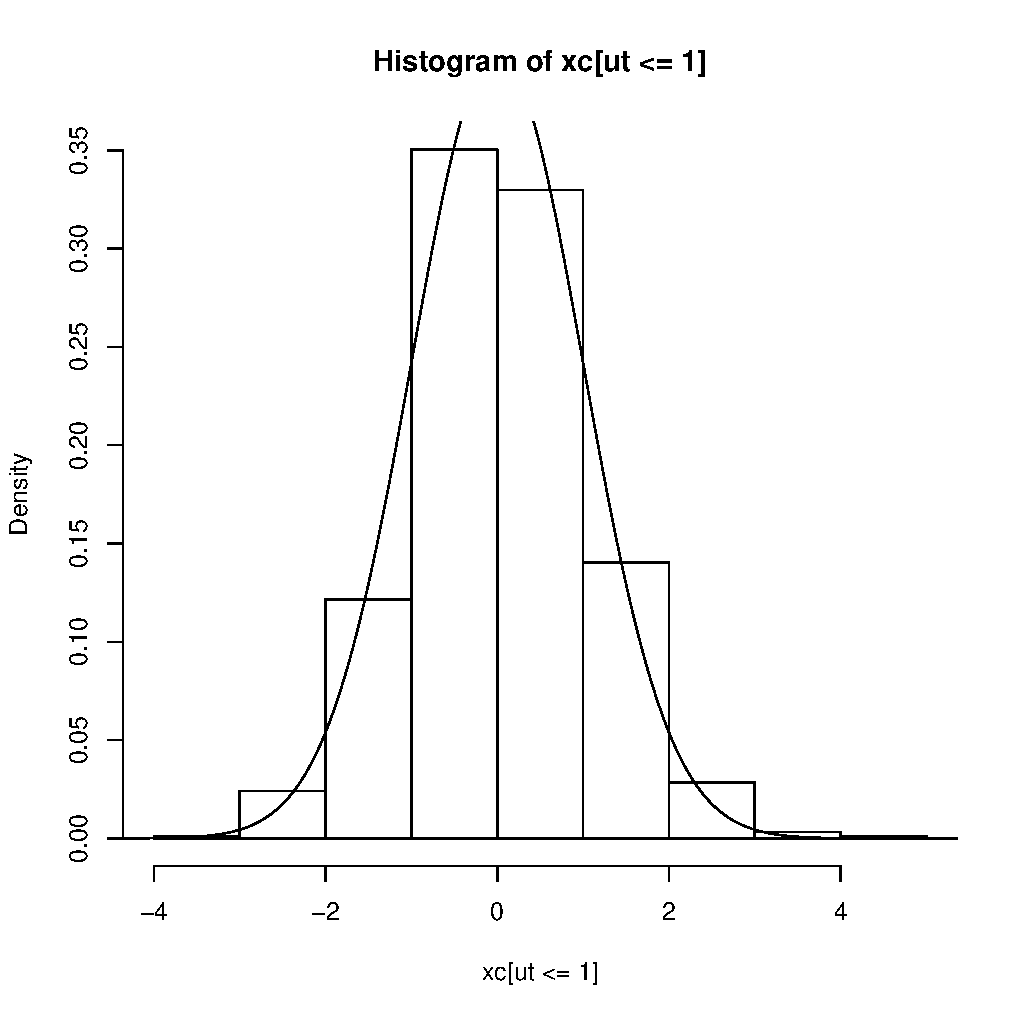
\includegraphics[scale=0.4]{1bq.pdf}
      \label{fig2}			
\end{figure}


\item The Chi Square Test was performed to test the goodness of fit to determine the 1000 samples generated.\footnotemark 
			\footnotetext{Refer Appendix 1c for the R code for goodness of fit}
The X- squared - 1000\\
df value - 999\\
p-value - 0.4851\\
Here the Null Hypothesis is not rejected.\\
 

\end{enumerate}





\item Question-2
\begin{enumerate}

\item The method of moments estimator for $\alpha$ is found by equating the first sample moment and E(X)\\
Thus,
			$$E[X]=\frac{\alpha}{\beta}=\frac{\sum{x_i}}{n}$$.
			$$\Leftrightarrow \hat{\alpha}_{MOM}=\beta\frac{\sum{x_i}}{n}$$
			Given $\beta=3.2$, the method of moments estimate for $\alpha$ was calculated to be 0.6859317.
\footnotemark 
			\footnotetext{Refer Appendix 2a for the R code used to compute the method of moment estimate.}\\

\item  The Maximum likelihood estimate for $\alpha$ was calculated to be  0.687098.The approximate 95\% confidence interval for $\alpha$, which was calculated using Bootstrapping and normal interval, is (0.6577010, 0.7164952).\\
Refer to Figure 3
\footnotemark 
			\footnotetext{Refer Appendix 2b for the R code used to compute the MLE .}
\begin{figure}[h]
	\caption[Figure 3]{Plot of MLE of $\alpha$}
    \centering
     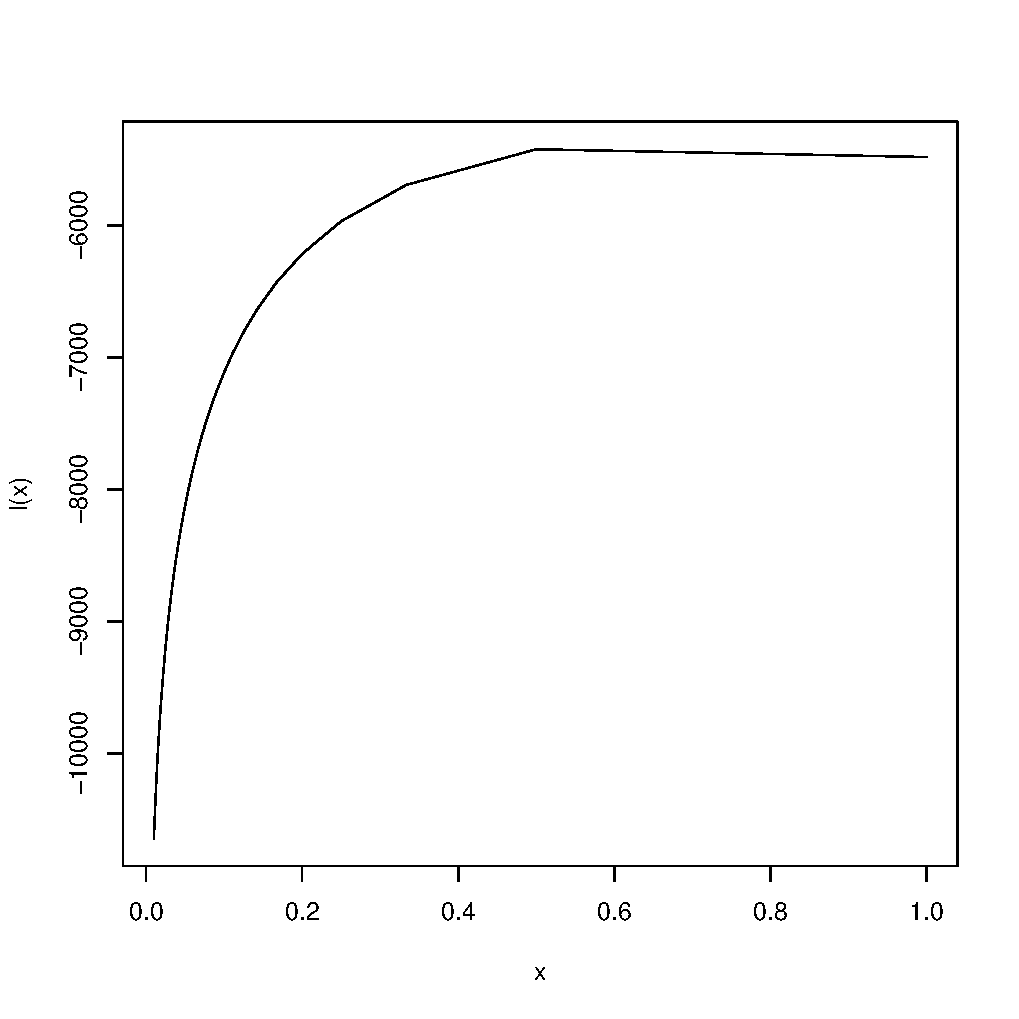
\includegraphics[scale=0.4]{2bq.pdf}
      \label{fig3}			
\end{figure}\\


\item The probability that a randomly selected policy has more than 2 claims in the year is $\pi=0.00306643$.\\ The  approximate 95\% confidence interval for $\pi$, which was calculated using the  Bootstrap Technique, is (0.01912874, 0.03139446).\footnotemark 
			\footnotetext{Refer Appendix 2c for the R code used to compute the estimator and the Confidence intervals.} \\
		

\end{enumerate}

\item Question 4
\begin{enumerate}
\item Theoretically, the probability of occurrence of HTT and HTH patterns occur are equal to $(\frac{1}{2})^{3} $.\\
Thus, the expected number of occurrences in \textbf{n} tosses=$n*(\frac{1}{2})^{3}$ \\
When we use simulation, the average number of tosses to obtain Pattern 1(HTH) is 7.22 and the average number of tosses to obtain Pattern 2 (HTT) is 10.13.\\
(Refer to Figure 4)\\
The results are surprising as they indicate higher average tosses for HTT than HTH because theoretically they must be equal.\footnotemark 
			\footnotetext{Refer Appendix 3a for the R code used to calculate the average number of tosses.} \\
\begin{figure}[h]
	\caption[Figure4]{Average Number of tosses for pattern 1 and pattern 2}
    \centering
     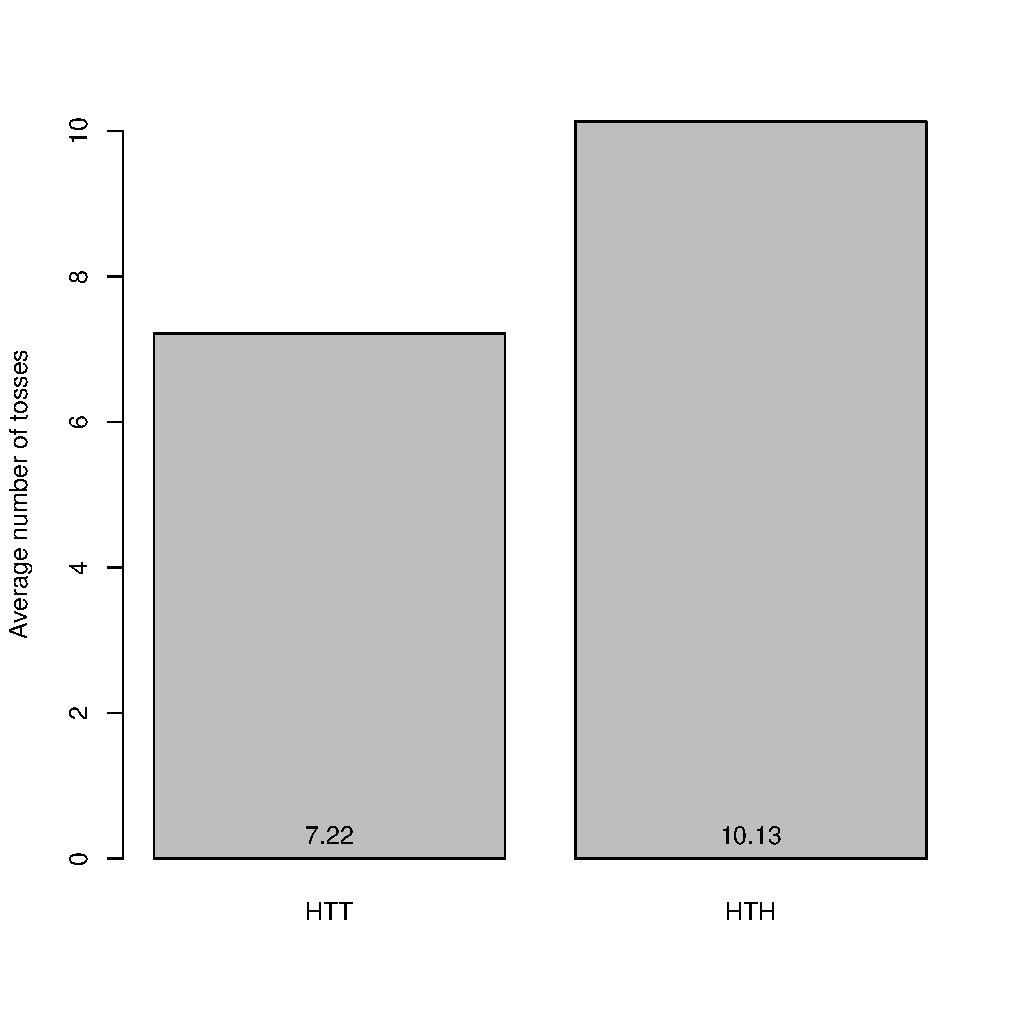
\includegraphics[scale=0.4]{3qa.pdf}
      \label{fig3}			
\end{figure}\\
 
\item


The number of occurrences of the HTH and HTT patterns in 100,000 trials are 9996 and 10010 respectively.
(Refer to Figure 5).
\footnotemark 
			\footnotetext{Refer Appendix 3b for the R code used to calculate the average number of tosses.} \\
\begin{figure}[h]
	\caption[Figure 5]{Number of occurences of Pattern1 and Pattern2}
    \centering
     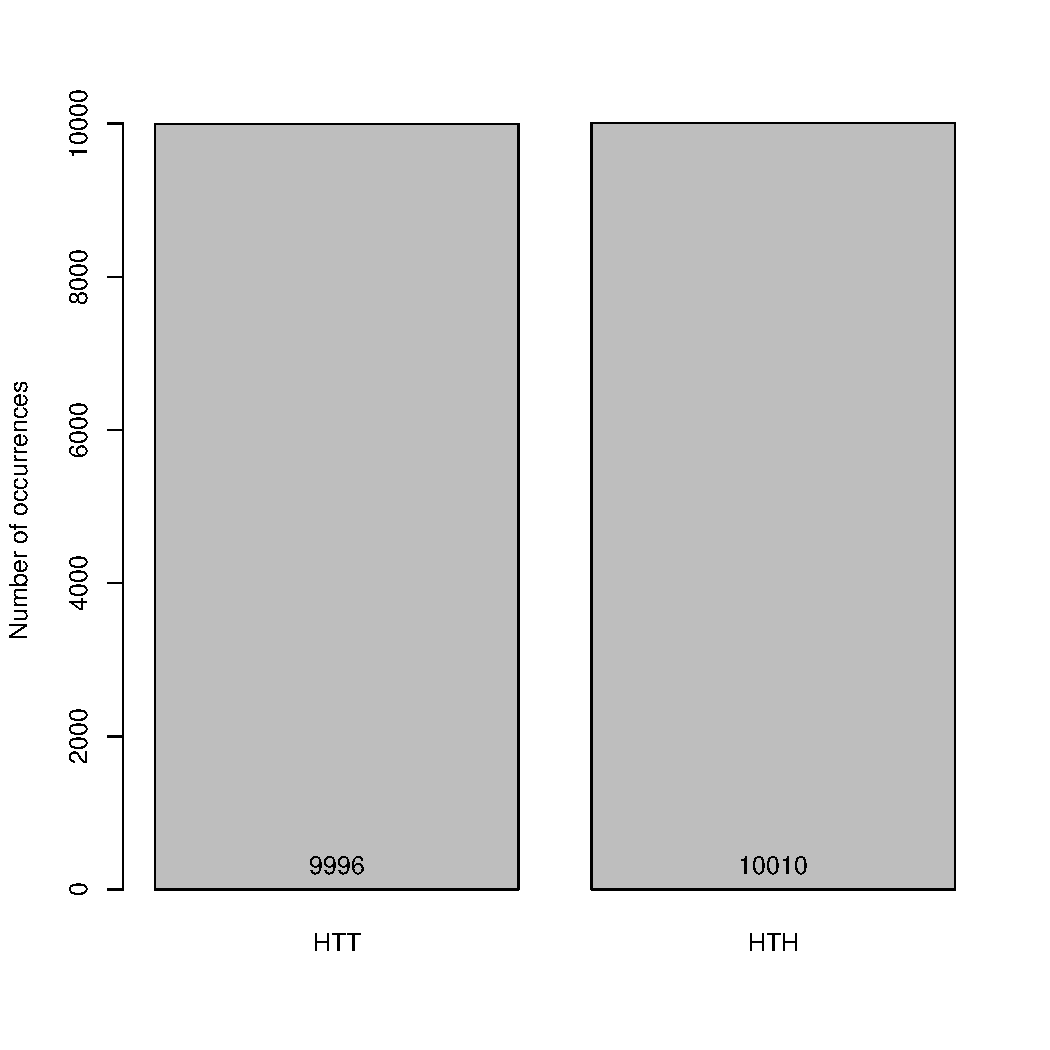
\includegraphics[scale=0.4]{3b.pdf}
      \label{fig3}			
\end{figure}\\


\end{enumerate}


\item Question 5

$X_{1},X_{2}......X_{n} ~ (a,5)$
\begin{enumerate}

\item
\begin{equation*}
f(x) \rightarrow
\begin{cases}
\frac{1}{b-a}\  if \ a <x<b\\\\
0   \ otherwise\\
\end{cases}
\end{equation*}\\

\begin{equation*}
= f(x) \rightarrow
\begin{cases}
\frac{1}{5-a}\  if \ a <x<b\\\\
0   \ otherwise\\
\end{cases}
\end{equation*}\\

$$\mu = E[X]$$\\

$$= \int_{a}^{5} x.f(x)$$\\ 

$$= \int_{a}^{5}  x.{\frac{1}{5-a}}dx$$\\

$$ = \dfrac{5+a}{2} = \bar X$$\\
Hence,

$$\hat a_{MOM} = 2\bar X - 5$$\\

\item
Maximim Likelihood Estimator of a\\

\begin{equation*}
f(x) \rightarrow
\begin{cases}
\frac{1}{b-a}\  if \ a <x<5\\\\
0   \ otherwise\\
\end{cases}
\end{equation*}\\

\begin{equation*}
L(x| a) =
\begin{cases}
\prod_{i=1}^{n}\frac{1}{5-a}\  if \ a < x < 5\\\\
0   \ otherwise\\
\end{cases}
\end{equation*}\\

\begin{equation*}
L(x|a) \rightarrow
\begin{cases}
{\frac{1}{5-a}}^n \  if \ a < x < 5\\\\
0   \ otherwise\\
\end{cases}
\end{equation*}\\

To maximize the L(x|a) , the value of (5-a) must be small and that is done using the min function.\\

$$a \leq min(X_{1},X_{2}......X_{n})$$
 
$$\hat a_{MLE} = min(X_{1},X_{2}......X_{n})$$\\

Hence,
$$\hat a_{MLE} = X_{(1)}$$\\


\item Maximum Likelihood Estimator of $\tau$

$$\tau = E[X] = \int_{a}^{5} x.f(x)dx$$\\
 Where,\\
 $$f(X) =frac{1}{5-a}$$\\
 So,
 $$= \int_{a}^{5} X. \frac{1}{5-a}$$\\
$$\dfrac{1}{2}( \dfrac{5^2-a^2}{5-a})$$\\
$$\tau =\frac{5+a}{2} \rightarrow \frac{5+X_{1}}{2}$$

\item

Here $\hat \tau$ is the MLE of $\tau$,\\
 and $\bar \tau$ is the methods of moment estimator of $\tau$ = E[X] \\
 a=1, and n= 10\footnotemark 
			\footnotetext{Refer Appendix 5d for the R code used to calculate the confidence intervals.} \\

 
 The coverage probability for a 95$\%$ confidence interval for$\tau$ was computed as:\\
 Normal CI :(2.76,3.43)\\
 Pivotal CI :(2.35,3.11)\\
 Percentile CI :(3.10, 3.91)\\
 
 The coverage probability for a 95$\%$ confidence interval for$\tau$ using $\bar \tau$:\\
 Normal CI :(1.88,3.39)\\
 Pivotal CI :(1.90,3.36)\\
 Percentile CI :(1.89, 3.39)\\
 
  


\end{enumerate}


\newpage
		\clearpage
		\fontsize{12}{12}
		\textbf{Appendix-1a}
		\fontsize{8}{12}
	\begin{verbatim}

 x<-seq(-10,10,length=100)
 opttheta <- function(x,theta){
    (sqrt(2/(pi*theta^2))*exp(-(x)^2+theta*abs(x)))
  }
 theta=1
 theta1=seq(0,2.5,0.1)
 opttheta1 <- function(theta1){
  (sqrt(2/(pi*theta1^2))*exp((theta1^2)/2))
  }

X11()
plot(theta1,opttheta1(theta1),type="l")
\end{verbatim}

		\fontsize{12}{12}
		\textbf{Appendix-1b}
		\fontsize{8}{12}
	\begin{verbatim}
func1 <- function(x,theta=1){
  x <- ((theta/2)*exp(-theta*abs(x)))/((1/(2*pi)^0.5)*exp((-x^2)/2))
  return(x)
  }

a <- (sqrt(2)/pi)*exp(.5)
xc <- rlaplace(1000,0,1)
uc <- runif(1000,0,1)
tc <-  a*sapply(xc, func1)
ut <- uc*tc

X11()
hist(xc[ut <=1], prob=T)
p<-ut <=1
p1<-rnorm(x)

X11()
hist(xc[ut <=1], prob=T)
p<-ut <=1
p1<-rnorm(x)

x=seq(-10,10,length=1000)
lines(x,dnorm(x))
sum(ut<=1)/1000

\end{verbatim}


\fontsize{12}{12}
		\textbf{Appendix-1c}
		\fontsize{8}{12}
	\begin{verbatim}
p<-ut <=1
p1<-rnorm(x)
chisq.test(p,rnorm(x))
\end{verbatim}


		\fontsize{12}{12}
		\textbf{Appendix-2a}
		\fontsize{8}{12}
	\begin{verbatim}
library(base)
 #Initializing given data
  data = c(rep(0,7840),rep(1,1317),rep(2,239),rep(3,42),rep(4,14),rep(5,4),rep(6,4),7)
 beta=3.2;

m=mean(data);
alpha.mom=m*beta;
alpha.mom
	\end{verbatim}
	
	\fontsize{12}{12}
		\textbf{Appendix-2b}
		\fontsize{8}{12}
	\begin{verbatim}
	data = c(rep(0,7840),rep(1,1317),rep(2,239),rep(3,42),rep(4,14),rep(5,4),rep(6,4),7)
beta=3.2;

logfn1 <- function (alpha){
  ba <- beta ^alpha
  dr <- (beta+1)^(alpha+data)
  return(-sum(log((ba)*gamma(alpha+data)/(factorial(data)*gamma(alpha)*dr))))
}
a <-c()
y <- c()
for(i in 1:100){
  a[i] <- 1/i
  y[i] <- logfn1(a[i])
}
z=-y
x11()
plot(a,z, xlab="x", ylab="l(x)",'l');
#finding the maximum of the function
mle_alpha <- nlminb(0.5,logfn1)$par
mle_alpha

fn <- function(alpha,data){
  ba <- beta ^alpha
  dr <- (beta+1)^(alpha+data)
  return(-sum(log(ba*gamma(alpha+data)/(factorial(data)*gamma(alpha)*dr))))
}

#finding confidence intervals
n=length(data);
B=100
mle_alpha_boot=c()
for(i in 1:B){
  boot_obs=sample(1:n,n,replace=T)
  y_boot = data[boot_obs] 
  for (j in 1:10)
  {
    a[j]=1/j
    y[j]=fn(a[j],y_boot)
  }
  mle_alpha_boot[i]=nlminb(0.5,fn,data=y_boot)[[1]];
}
se = sqrt(var(mle_alpha_boot))
#Calculating the Normal confidence interval
Normal = c(mle_alpha_boot-2*se, mle_alpha_boot+2*se)

	\end{verbatim}


\fontsize{12}{12}
		\textbf{Appendix-2c}
		\fontsize{8}{12}
	\begin{verbatim}
	n=length(data);
#calculating the observed probability of more than 2 claims  
          prob <- data[data[]==2]
          prob <- length(prob)/n;
#finding confidence intervals using Bootstrap technique

prob.boot=c();
pb=c();
for(i in 1:100){
  x <- sample(1:n,n,replace=T)
  x.bootstrap <- data[x] 
  pb <- x.bootstrap[x.bootstrap[]>2]
  prob.boot[i] <- length(prob.boot)/n;
}
serror = sqrt(var(prob.boot))

#Calculating the Normal confidence interval
Normal = c(prob-2*serror, prob+2*serror)

	\end{verbatim}



\fontsize{12}{12}
		\textbf{Appendix-3a}
		\fontsize{8}{12}
	\begin{verbatim}
	#Creating two column vectors of size 100 with all values 3. 
    X1=c(rep(3,100))
    X2=c(rep(3,100))
for(i in 1:100)
{
  #let X1[i] be the variable to count the number of trials to get  HTT at the ith trial
  y=round(runif(X1[i],0,1))
  while((y[X1[i]-2]!=1)||(y[X1[i]-1]!=0)||(y[X1[i]]!=0)) # checking for pattern 1
     {
        X1[i] <- X1[i]+1;
        y[X1[k]]<- round(runif(1,0,1))
     }
  
  #let X2[k] be the variable to count the number of trials to get  HTH at the kth trial
  y=round(runif(X2[i],0,1))
  while((y[X2[i]-2]!=1)||(y[X2[i]-1]!=0)||(y[X2[i]]!=1)) # checking for pattern 2
  {
        X2[i] <- X2[i]+1;
    y[X2[i]] <- round(runif(1,0,1))
  }
}
#Gives mean number of tosses required to observe each pattern
pattern1 <- mean(X1)
pattern2 <- mean(X2)

figure <- barplot(c(pattern1,pattern2), names.arg=c("HTT","HTH"),ylab="Average number of tosses")
text(figure,0,c(pattern1,pattern2),cex=1,pos=3)
\end{verbatim}

\fontsize{12}{12}
		\textbf{Appendix-3b}
		\fontsize{8}{12}
	\begin{verbatim}
x=round(runif(100000,0,1));
a=0;
b=0;
#Checking for Patterns HTT and HTH
for(i in 3:100000)
{
  if((x[i-2]==1)&(x[i-1]==0)&(x[i]==0))
    a=a+1
  if((x[i-2]==1)&(x[i-1]==0)&(x[i]==1))
    b=b+1
}
figure=barplot(c(a,b), names.arg=c("HTT","HTH"),ylab="Number of occurrences")
text(figure1,0,c(a,b),cex=1,pos=3)
\end{verbatim}

\fontsize{12}{12}
		\textbf{Appendix-5d}
		\fontsize{8}{12}
	\begin{verbatim}
library("base")
x<-runif(10,1,5)
i=1
for(i in 1:100)
{
  boot <- sample(seq(1:10),10,replace=T)
  x.boot <- x[boot]
  mle.a <- min(x.boot[])
  mle.tau <- (5 + mle.a)/2
  tau <-(5+1)/2
  mom.tau <- (5+2(min(boot.obs)-5))/2
}
Normal = c(tau-2*se, tau+2*se)
pivotal = c(2*tau-quantile(x.boot,.975),2*tau-quantile(x.boot,.025))
percentile = c(quantile(x.boot,.025),quantile(x.boot,.975))
Normal1 = c(mom.tau-2*se, mom.tau+2*se)
pivotal1 = c(2*mom.tau-quantile(x.boot,.975),2*mom.tau-quantile(x.boot,.025))
percentile1 = c(quantile(x.boot,.025),quantile(x.boot,.975))

\end{verbatim}







\end{enumerate}
\end{document}